\chapter{System Evaluation}
The final product has all its intended functionality. Horton is robust and quick, while Repota is user-friendly and has met all the required features. Horton was tested thoroughly through integration testing with the tests package from Go. Repota's functionality was verified through high-level behaviour tests with CucumberJS (JavaScript). In order to perform these tests, a mock database was constructed especially for these processes. The reason for a mock database was to avoid conflict with the production database and avoid affecting the real data of users and reports.

\section{Horton Robustness}
The tests package from Go was used to test all of Horton's functions for the Routers, Account, Session, and Reports Systems and the data request from Back4App. The tests consist of HTTP methods to either check if everything is up and running, get data, or send payloads of data with the models (Figure 5.1) to the respected endpoints (Figure 5.2). The tests pass on the conditions of the response status codes and messages. For example, a '200 OK' would be a pass, and '500 Internal Server Error' would be a fail (Figure 5.3).

\begin{figure}[H]
    \centering
    \caption{Payload of mock user details}
    \label{image:registertest}
    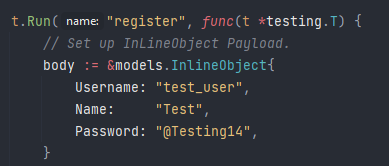
\includegraphics[width=0.6\textwidth]{images/horton/tests/register_test_payload.png}
\end{figure}

\begin{figure}[H]
    \centering
    \caption{Test Register - POST request}
    \label{image:registerTestPostReq}
    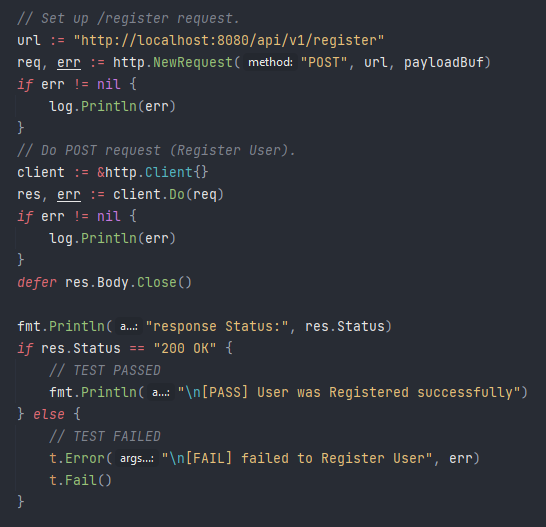
\includegraphics[width=0.8\textwidth]{images/horton/tests/test_register_post.png}
\end{figure}

\begin{figure}[H]
    \centering
    \caption{Register test pass}
    \label{image:registerTestPass}
    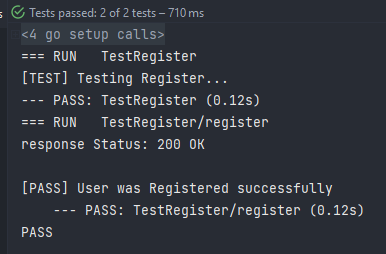
\includegraphics[width=0.8\textwidth]{images/horton/tests/register_test_pass.png}
\end{figure}

\section{Repota Robustness}
CucumberJS was used throughout Repota to run through the app and test its high-level behavior of the features register, login, logout, create, edit and delete a report from a user's perspective. There are two sides to Cucumber, the Gerkin features, and the step definitions. Features consist of 'User Stories' and a 'Scenarios' (Figure 5.4). A User Story includes the name of a feature to test, the possible stakeholder, and the feature's need. Scenarios are the steps required to test the app's feature. Step definitions then perform these steps (Figure 5.5). The steps for the tests include navigation throughout the app to test multiple features at one time. All the tests were done through a controlled Firefox with Selenium WebDriver. The tests pass on a count of all the steps begin completed successfully (Figure 5.6).

\begin{figure}[H]
    \centering
    \caption{Login Feature}
    \label{image:loginFeature}
    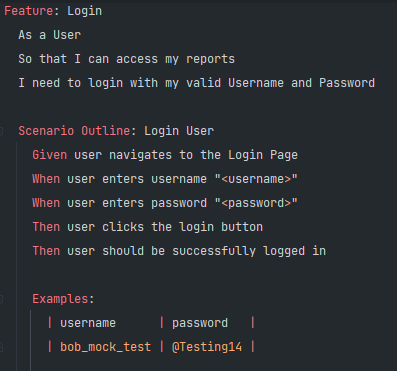
\includegraphics[width=1.0\textwidth]{images/repota/tests/login_feature.png}
\end{figure}

\begin{figure}[H]
    \centering
    \caption{Login Steps}
    \label{image:loginSteps}
    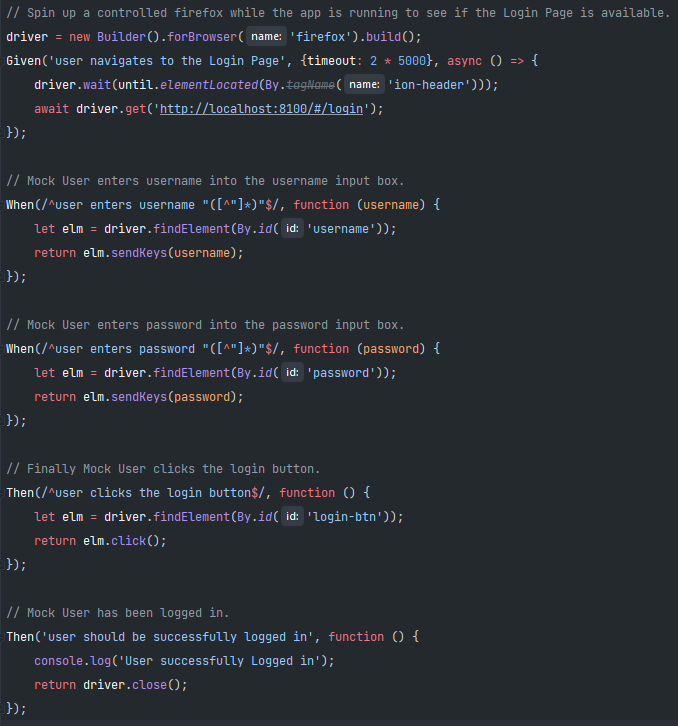
\includegraphics[width=0.8\textwidth]{images/repota/tests/login_steps.png}
\end{figure}

\begin{figure}[H]
    \centering
    \caption{Login Steps Pass}
    \label{image:loginStepsPass}
    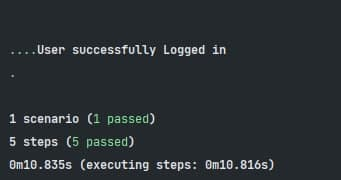
\includegraphics[width=0.8\textwidth]{images/repota/tests/login_pass.png}
\end{figure}

\section{Mobile Phone Functionality}
Repota was tested for its functionality on Android through Chrome's DevTools. The DevTools was primarily used to check if all requests were successful in verifying all the features were working. Another vital check was especially to ensure cookies were being set on mobile phones as the app relies heavily on them.

\begin{figure}[H]
    \centering
    \caption{Repota on Chrome DevTools}
    \label{image:devTools}
    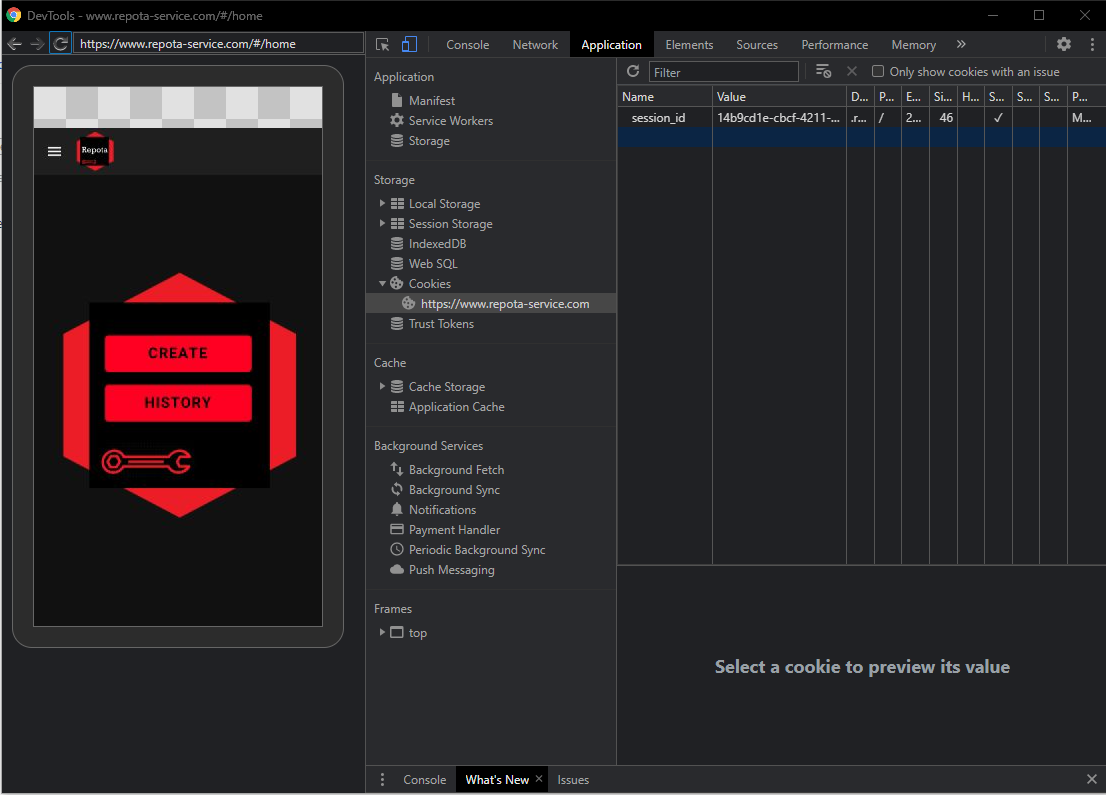
\includegraphics[width=1.0\textwidth]{images/repota/tests/repota_devTools.png}
\end{figure}

\subsection{Responsiveness}
Repota is responsive on multiple devices. Ionic Lab helped to achieve this immensely. The app's responsiveness has been tested on the browsers Google Chrome, Firefox and Microsoft Edge. While for mobile phones, it was tested on Android and iPhone. The figure below shows a screenshot of the app's create page on a Google Pixel 3a with the Chrome app.

\begin{figure}[H]
    \centering
    \caption{Repota on Mobile Phone}
    \label{image:mobileHome}
    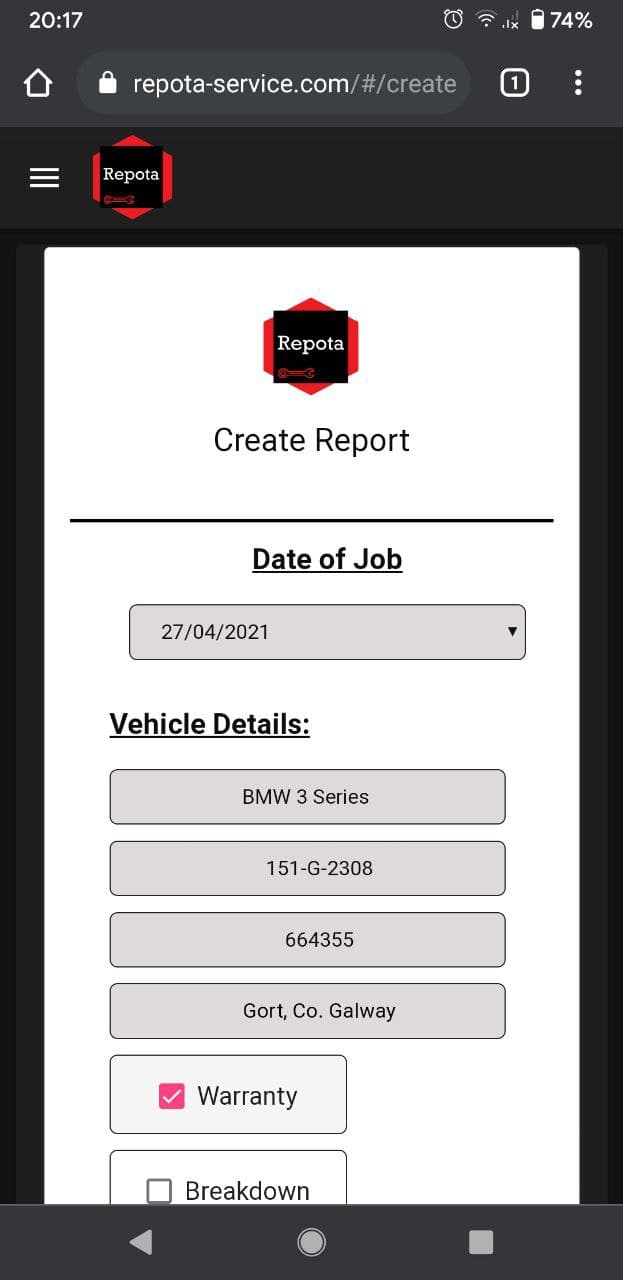
\includegraphics[width=0.6\textwidth]{images/repota/UI/create-mobile-phone.jpg}
\end{figure}

\newpage
\section{Issues Encountered}
This section goes over the issues encountered that caused long pauses in the development of Repota.

\subsection{Cookies}
Browser cookies were quite challenging to get set on the front-end. The initial cookie setup for a logged-in user could not cross over to the front-end from the back-end. This issue did baffle me for quite some time. The debugging DevTools for browsers indicated a warning that said a SameSite had to be specified. This misled me into altering how the cookie was set. However, Gin Gonic's documentation states that, a SameSite of 'None' is set by default. In the end, it came down to a CORS requirement for  'Access Control Allow Origin'. Originally I had '*' specified as a wildcard for any origin. The wildcard had to be changed to the request, header key 'Origin' to resolve this issue.

\subsection{Export to PDF}
The initial library used for exporting reports to PDFs was html2pdf. The PDF was of excellent quality for computers and mobile phones. Unfortunately, due to Angular's stylesheets connected to multiple pages, html2pdf caused a DOM (Document Object Body) Exception for "Sharing constructed stylesheets in multiple documents is not allowed." This exception caused the hamburger menu button to disappear. Many attempts were made to catch the exception and prevent it. As a last resort, I went to the extreme of disconnecting the Export Page from all the stylesheets and had the CSS right in the HTML, and this did not change anything. I did find a solution for this exception for html2canvas on one of the issues on the html2canvas GitHub Repository. I attempted to translate the solution for html2pdf with no success. Then I created an issue on the html2pdf GitHub Repository. Shortly after this, I came across the libraries dom-to-image and jsPDF. This setup for the PDF caused no exceptions. On computers, the PDF comes out just as expected. However, on mobile phones, the reports comes out half the size of the PDF. Again I made attempts to have the PDF requirements resize when on mobile phones, but this resulted in the report being squashed on the PDF. All this resulted in having only the PDFs exported on computers to have an acceptable format. I got no response for the issue on the html2pdf GitHub Repository. It was then seen that it was better to have the export to PDF working right on one device rather than two devices with a DOM exception.

\subsection{Finding the right 3rd Party API}
Finding the right 3rd party API was not a straight forward process. Two other APIs were tried and tested before discovering Back4App. The first one found is called VINCARIO. I had to request an API key from them. They accepted the request and sent code examples to use their service in Python, PHP and Node.js. I was able to translate the Python example to Go and they asked me for the code so they could have it for other users wanting to use their service with Go and I happily sent it on to them. Once the code was in place it was realised this API has access to only one vehicle at a time. This limitation ruled it out as a very large function or a loop would have been needed to get multiple vehicles at one time. The second is named Car Makes and Models Database API. This API has access to more than one vehicle at time but they require one credit for each request. I was given twenty credits to start off with but this soon ran out and I attempted to pay for more credits but the API's PayPal service was down and still is months later. I contacted them to let them know it was down and I received no response. As a result this API was ruled out too. Some more research and exploring was done and Back4App was finally discovered which, suited the needs perfectly. 


